\chapter{Background}
\label{chap:bg}
This chapter is divided into two sections. The first one, \ref{sec:ThB} Theoretical Background, will provide a description of a simple CPU architecture whit focus on the parts used for executing memory instructions (loads and stores). This will be followed by a introduction of the four already implemented prefetching strategies. Section~\ref{sec:TWF} will go thought the work flow of this thesis and introduce the tools that are used, modified or created, as well as how they are combined.
\section{Theoretical Background}
\label{sec:ThB}

\subsection{A theoretical Architecture}
\label{subsec:TA}
\begin{figure}[h]
\centering
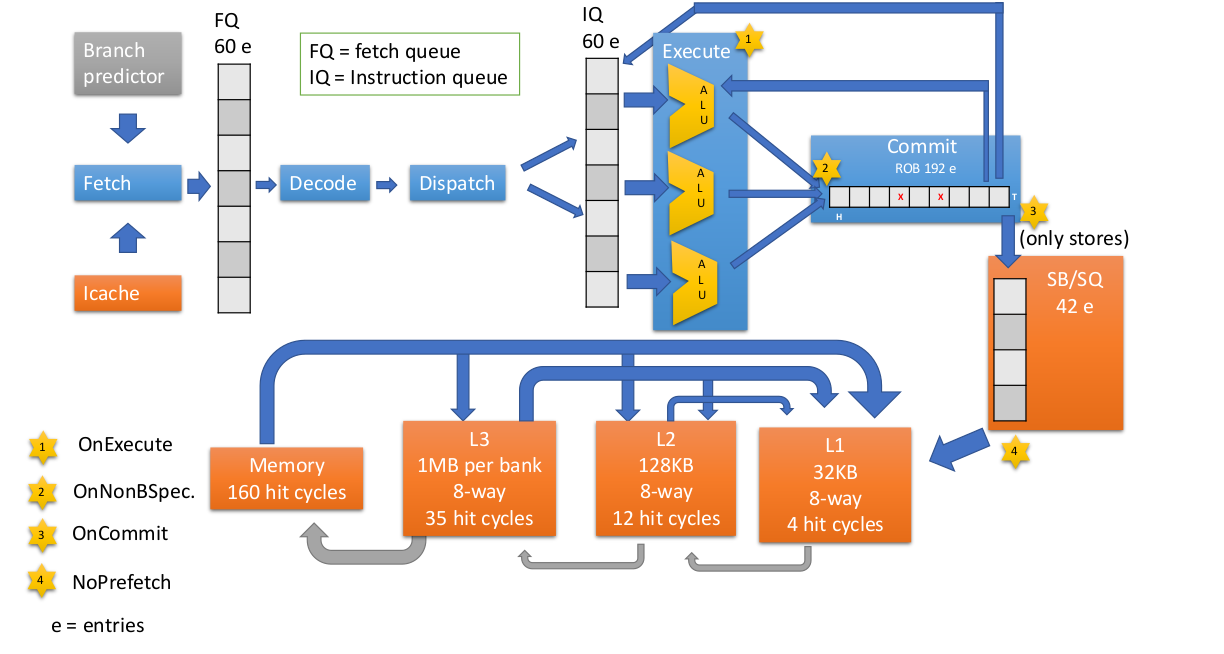
\includegraphics[width=8cm]{figure/thoeratical-arc.PNG}
\caption{A theoretical architecture}
\label{img:arc}
\end{figure}
In modern CPU's there are often more then one cores which all have a process pipeline with several stages. The pipeline is slitted in stages to increase the thought put of executed instructions. One can compare it with a car factory where the car travels on a conveyor belt thought different stations, on each station something is done with the car, i.e. seats, wheels or the engine can be installed. Here we have a six stage pipeline (see the top of the image~\ref{img:arc}). The six stages are:
 \begin{itemize}
   \item \textbf{Fetch.} A new instruction (see \ref{subsec:tarce}) will be added to the pipeline.
   \item \textbf{Decorde.} The instruction will here be interpreted.
   \item \textbf{Alloc.} Needed registers (memory within the actual core of the CPU, to make arithmetical operation the data has to be placed in one register by a previous load instruction) are allocated
   \item \textbf{Issue.} ??
   \item \textbf{Execute.} Here is the actual work done i.e. compute a memory address. 
   \item \textbf{Commit.} The hand-over stage where the CPU places a load instruction in the load buffer or a store instruction in the store buffer. We will soon come back to theses buffers. 
 \end{itemize}
 The memory structure (in the center of image \ref{img:arc}) is of course a key part when talking about memory instructions. We begin with the main memory that have a storage capacity of some gigabytes (GB) and sits on the mother board. Then we have the cashes, which are placed on the CPU chip. In this case we have two but three are also common, there are named L1, L2 and L3. Where L stands for level and the grater the digit is the  bigger the cash is and the further away from the core it is placed. A bigger cash means that it takes longer time to find certain data in it. When data is loaded into the L1 cash from the main memory it will often be loaded to all the other cashes at the same time. 
 \\ \\
 Now back to the two buffers, to the upper left in the image~\ref{img:arc} you will see a store buffer (the load buffer works in the same way and  have therefore not been painted). The memory address to be fetched and, if a store, the data to be stored will be placed in the store or load buffer on commit. The buffers are FIFO-ordered (first in first out), the first load in the buffer sits and wait for its data to be ready in the L1 cash and blocks all operations behind in that buffer. This is the same for the store as well and means that the buffer only interact with the L1 cash.
\subsection{The given prefetch policies}
\label{subsec:GPP}
The question for this master thesis is when to prefetch data into the L1 cash to minimize the time a memory instruction has to wait in the first place of a buffer. Four approaches are already implement in the Gems simulator~\ref{subsec:gems} and these will be described and there pros and cons while be mentioned below, based on the architecture introduced in section~\ref{subsec:TA}. From now on we will for simplicity only talk about stores but the word "store" can just be replaced with "load". \\

\paragraph{OnExecute}\label{per:ONEX} \textbf{Gharachorloo, ISCA 91.} This is the earlies and most speculative one, where the operation to brought memory into the L1 cash is issued in the execute stage. This ensure the data to arrive in L1 before it is needed, i.e. its instruction is first in the buffer. The down side is that several things with impact on the data to be prefetch can occur. First, if the store instruction is affected by a branch, that branch can turn to be miss predicted which means that we waste energy and space in the small L1 cash by bringing in unneeded data. Bringing in data to a cash can cause an eviction of other data. If a store instruction arrives to the first place in the buffer and found that its data have been evicted from the L1 cash it have to wait for the data to be brought to the L1 again. This will hopefully take less time since the data can be left in the L2 cash and be brought from it instead of the main memory. Given that the prediction is right we might still be in trouble, since when we issue the prefetch, the instruction have to finish the pipeline and passes thought the queue in the buffer. This might take long time. During that time the data can have arrived to the L1 buffer and been evicted due to lack of space since more data can have been prefetch from the point in time it arrives in L1 until the instruction for it is first in the buffer. A too early prefetch can also be a vulnerability since malicious software can cause a prefetch of illegal data before the core figures out that it is illegal, and when it does the data can already have been exposed. To conclude one can says that this alternative is the best if nothing goes wrong but it is a lot of things that can go wrong.

\paragraph{OnCommit} \label{per:ONCO} \textbf{Intel cores} Here the prefetch is issued in the commit stage (then passing the instruction to the store buffer). This means that will not prefetch unneeded data. There are still a possibility that the data while be brought in and evicted due to lack of space, while waiting, as describe in the previous paragraph~\ref{per:ONEX}. Prefetching data on commit might still mean that the instruction may be waiting in the first line of the buffer. This can, in the worst case, fill up the entire buffer which can stall the processor i.e. block it from executing any other instruction. To conclude, OnCommit is the man in the middle between the two extremes, OnExecute~\ref{per:ONEX} and NoPrefetch~\ref{per:NOPR}.

\paragraph{NoPrefetch} \label{per:NOPR} \textbf{Gem5?}. Here we have no prefetch, the data with be brought into the L1 cash then the instruction is first in the buffer. The data we brought will be needed and not evicted before use. We will waste no energy. The down side is that every instruction will be blocking the buffer for a long time waiting on its data to become available in the L1 cache. The risk for filling up the buffer and stall the processor (see~\ref{par:ONCO}) is high. To conclude this is the most energy efficient but the most time consuming trade of.

\paragraph{OnNonBSpeculative} \label{per:ONBS} This alternative is proposed by Albert Ros Bardisa (the supervisor of this master thesis) and has not been implement nor test in a brighter setup, it is only implemented in the Gems simulator~\ref{subsec:gems}. The alternative can be seen of as taken the best of OnExecute~\ref{per:ONEX} and OnCommit~\ref{per:ONCO}. If you have a load instructive that are effected by a branch we will wait until the outcome of the branch is know, we will make sure that all data we bring in to the L1 cash will be needed. We act as OnCommit. If the load is not effected by a branch we will then benefit on the performance by acting like OnExecute~\ref{per:ONCO}.  






\section{The work-flow}
\label{sec:TWF}
\begin{figure}[!h]
\centering
\begin{tikzpicture}[thick]
  \node[draw,rectangle] (a) {Program};
  \node[draw, ellipse,right of=a,  node distance=2cm] (b) {Sniper};
  \node[draw,rectangle,above of=b,  node distance=1cm] (c) {Configuration};
  \node[draw,ellipse,right of=b,  node distance=2cm] (d) {Trace};
  \node[draw,ellipse,right of=d,  node distance=2cm] (e) {Gems};
  \node[draw,ellipse,above of=e,  node distance=1cm] (f) {CPU architecture};
  \node[draw,rectangle,right of=e,  node distance=2cm] (g) {status-files};
  \node[draw,circle,below of=e,  node distance=2cm, text width=4em, text centered] (h) {Python scripts};
  \node[draw,circle,left of=h,  node distance=3cm, text width=4em, text centered] (i) {graphs \&  tables};
  % 1st pass: draw arrows
  \draw[vecArrow] (a) to (b);
  \draw[vecArrow] (c) to (b);
  \draw[vecArrow] (b) to (d);
  \draw[vecArrow] (d) to (e);
  \draw[vecArrow] (f) to (e);
  \draw[vecArrow] (e) to (g);
  \draw[vecArrow] (g) |- (h);
  \draw[vecArrow] (h) to (i);


  % 2nd pass: copy all from 1st pass, and replace vecArrow with innerWhite
  \draw[innerWhite] (a) to (b);
  \draw[innerWhite] (c) to (b);
  \draw[innerWhite] (b) to (d);
  \draw[innerWhite] (d) to (e);
  \draw[innerWhite] (f) to (e);
  \draw[innerWhite] (e) to (g);
  \draw[innerWhite] (g) |- (h);
  \draw[innerWhite] (h) to (i);
 

  % Note: If you have no branches, the 2nd pass is not needed

\end{tikzpicture} 
\caption{An overview of the work process and the parts involved.  The rectangles are existing parts, ellipses are modified parts and circles are new parts (created within this thesis)}
\label{chart:workProcess}
\end{figure}
\subsection{Program}
\label{sec:program}

\subsection{Sniper}
\label{sec:sniper}

\subsection{Configuration}
\label{sec:conf}

\subsection{Trace}
\label{subsec:tarce}

\subsection{Gems}
\label{subsec:gems}

\subsection{CPU architecture}
\label{sec:architecture}

\subsection{Python scripts plus graphs \& tables}
\label{sec:architecture}

